%%This is a very basic article template.
%%There is just one section and two subsections.
\documentclass{article}
\usepackage[utf8]{inputenc}
\usepackage{hyperref}
\usepackage{pdfpages}
\usepackage{pdflscape}
%\usepackage{natbib}
\usepackage{bibentry}
%\usepackage[backend=biber,style=coppe]{biblatex}
\begin{document}
\nobibliography*

\title{Master Thesis Proposal - Underwater Mapping Using Imaging Sonars}
\author{Eduardo Elael de M. Soares}

\maketitle
\tableofcontents

\section{Introduction}

This proposal refers to a system for 3D underwater mapping. It consists of a
hardware plus a software that is the main objective of the research. The
chosen hardware will constrain the software options and decisions on the
underling algorithm.

A mapping system usually comes together with a localization algorithm in what is
called a SLAM (\textit{Simultaneous Localization and Mapping}). SLAM is an
active topic of research and has remarkable solutions using laser scanners,
%http://www.frc.ri.cmu.edu/~jizhang03/Publications/RSS_2014.pdf
%http://www.frc.ri.cmu.edu/~jizhang03/Publications/IROS_2014.pdf
but most of the underwater SLAM is focused on 2D maps treating the environment
as a floor plant or as 2.5D maps of the seafloor.

The reason for the problematic of underwater mapping, and thus SLAM, in contrast
with laser based systems used outside water is mainly its sensor. While lasers
are precise low-noise sensors, sonars, which are the standard sensor for
underwater SLAM, are the opposite.

Sonars measures the sound on the water, its main parts are the hydrophones. They
can emit and receive sound waves just like microphones and headphones do in the
air. They can be specialized to listen the environment and interpret its sounds,
usually by their spectrum, which is the case for passive sonars. Or they can
emit a beam of sound and wait for the reception of the echo.

 When talking about active sonars, the ones that measures sound echo emitted
by itself, there are two important classes based on its beam directional gain:
Profiling and Imaging.

Profiling have a narrow pencil shaped beam, with an aperture of about $1.7$
degrees, i.e. the half power point. It is meant to have a similar response of
what is expected from a laser scanner, but working with sound waves. At the end
of the day, they does not correlate much because they differ greatly on noise,
response time and spatial resolution.

Imaging sonars will be the focus of this work, they make use of a much wider
than Profiling sonar fan shaped beam. It use to have around $3$ degrees angle of
aperture in the vertical direction, but keeping same angular resolution on the
horizontal plane.
It does not have to precisely aim to provide a localized information about the
target, but rather a more general information, being able to infer some information
about the presence of objects below or above its horizontal plane. From this
point of view, each beam gives a concentrated information about the region it
ensonifies, so fusing the information of multiple beams from different
directions and angles is expected to give a better outline of the environment
than just using isolated sonar responses.

Besides classification based on beam shape, there are others as multi- or single
beam. Firing multiple beams at once gives a faster rate, as one does not need to
wait for the response to arrive before redirecting the beam to the next angular
position. But the least expensive still single beam and is the one that is going
to be considered.


\section{Motivation}

The mapping of underwater environments is not just a part of a SLAM system. It
might have importance on its own, it can be used for humans to visualize things
that could not be seeing otherwise. 

In the ROSA (\textit{Robô para Operações de Stoplogs Alagados}) project,
developed by LEAD/COPPETEC to ESBR, one of the goals is to make a reconstruction
of the hydroelectric power plant turbine entrance to spot any underwater debris
that could block the lowering of stoplogs, used to block the water flow, and
then cause delays and setbacks. When it happens for a stoplock to stuck the need
for a diver also incur in further human risk, so even then it is important to
know the surroundings.

On a developing perspective, besides the importance for the ROSA project, it has
characteristics that makes it appropriate for mapping. It has a lifting beam for
inserting the stoplogs into the water that can act as stable fixation point for
any sonar structure. So reducing the impact of poor a localization system on the
mapping. It also has a known and not-so-complex ground truth environment
(besides possible debris). Thus data collected there is suitable for testing the mapping
algorithm in a real world environment, as opposed to lab testing.
Although the noise environment might impair greatly the mapping, and subsequent
visual reconstruction.


It is also a integral part ROV's, where it gives feedback to the operator for
him to know where it is or/and what he is doing, especially because cameras do
not have a very useful range. And glaringly its automated counterpart (AUV's) as
a requisite for SLAM.



\section{Objectives}

The general objective is to map an underwater environment. But to get there it
is important to describe some facts first.
 
As stated before, profiling sonar try to mimic laser scanner, but using sound.
So most of the approaches on 3D underwater SLAM focus on applying laser scanner
techniques to profiling sonars, e.g. point cloud reconstruction. On the other
hand, imaging sonars are usually cheaper and gives more information per sound
beam. So having the possibility of using imaging sonar and benefiting from its
extra information is a win-win strategy.

Besides the definition of the sonar, one should carefully look into the meaning
of mapping, because, it can be interpreted in different ways, depending on the
context.
Taking what they all have in common, it is possible to generically define
mapping as being the processing of received environmental data to characterize
the surroundings. In the understanding of characterization is where the
difference lays, how the environs are going to be represented is dependent on
the application.

On a SLAM system there is no intrinsic need for a human readable map. In such a
system, it may be more interesting to store the map information, the
\"characterization\", only through its most representative features, if that is
what matters for the localization procedure.

Still, if the map is to be seen by a human it should store more
information about the environment, so that it can be displayed as a usual map,
3D or 2D depending on the case. This representation also guides how the data
could be stored, e.g. if it wants to show a surface, it can be stored as a
elevation map, or if one wants to see a 3D object it can be stored as a point
cloud.

Using de aforementioned ideas, the main goal of the thesis reported here is to
implement state of the art techniques for mapping, using binary bayesian
filters. Fuse all the data on a octree structure using a robotic framework,
named ROCK, and implement a visualization for the reconstruct underwater map.
The data source shall be a imaging sonar mounted on a pan-tilt unit, so
to provide the sonar extra degrees of freedom.

Optimization of the visible surface for based on the expected response of a
sonar beam in a given direction will also be attempted. It might supply
information about the surface material, specifically its reflectance. A
technique based on previously articles.


\section{Metodology and Expected Results}

The work is divided into tree main branches. Each having a theoretical research
followed by implementation and testing.

The sonar model definition starts with a compilation on the description of sound
waves on the water, reflection, sonar directional gain and noise sources. Then
tests are realised on known environments so to fit and validate the proposed
model. The test results are finally used create the full sonar model, including
metric conventions by the sonar protocol.

The second branch deal with the map filling, basically the Binary Bayesian
Filter implementation. A review on Bayesian Filtering is scheduled before the
coding writing to be done on the robotics framework, ROCK. The implementation
will make use of the Octotree data structure, through the Octomap library, to
store the map.

The integration of the sonar model with the Bayesian Filter give the means to
process sonar data. So data acquired on the LNDC/UFRJ tank (Laboratório de
Ensaios Não Destrutivos, Corrosão e Soldagem), which loosely translated means
 Non-Destructive Testing, Corrosion and Welding Laboratory, and on the Jirau
 Power Plant, by means of the ROSA/COPPETEC project, will be processed and
 compared to the tank and power plant entry layout, respectively. 
 
 In a more complex endeavor, which is the third branch, a theoretical derivation
 for the optimization of 2D surfaces embed on 3D environments will take place.
 It uses sonar response as expectation, and must take into account the
 probabilistic nature of the map grid. The objective is, instead of having a
 fixed sonar model, be able to better infer the underlying geometry of a sonar
 responde, and also recover some information about the surrounding materials
 reflectivity properties. This optimization algorithm will then be implemented
 on ROCK so it can also be integrated to the Bayesian Filter, instead of the
 sonar model. The same data processed by the combination ``Filter + Sonar
 Model'' shall now be processed by ``Filter + Optimization''.
 
 Based on the literature, even with not much similar works, the reconstruction
 with \textit{a priori} sonar model will probably experience problems when
 reconstructing corners, shallow angle surfaces, very complex (intense
 multipath) or on highly noise environments. For the optimization, it shall
 encounter similar issues, but a less accentuated shallow angle quality
 degradation and an overall less blurry reconstruction.

\section{Proposed Bibliography}



\subsection{Physics of Sound}
\begin{itemize}
  \item \bibentry{Etter2013}
  \item \bibentry{Ziomek1993}
  \item \bibentry{Scheipers2010}
  \item \bibentry{Kagawa2001}
  \item \bibentry{Tsuji2002}
  \item \bibentry{KjaerBruel2014}
  \item \bibentry{FrohlichJuliaandWachsmuth2011}
  \item \bibentry{Michalis2011}
  \item \bibentry{Nironen2004}
  \item \bibentry{Wand2003}
\end{itemize}

\subsection{Math Background}
\begin{itemize}
  \item \bibentry{Barshan2007}
  \item \bibentry{Christakos2002}
  \item \bibentry{Blanco2008}
  \item \bibentry{Choset2005}
  \item \bibentry{Approach}
\end{itemize}

\subsection{Mapping Techniques}
\begin{itemize}
\item
\bibentry{Sun2008}  \item \bibentry{Hu2012}  \item \bibentry{Coiras2009}  \item \bibentry{Thrun2002}  \item \bibentry{Pidsley1995}  \item \bibentry{Ribas2006}  \item \bibentry{Coiras2007}  \item \bibentry{Pagac1998}  \item \bibentry{Hernandez2009}  \item \bibentry{Mallios2009}  \item \bibentry{Lim1992}  \item \bibentry{Zerr1996}  \item \bibentry{Rosenblum1992}  \item \bibentry{Moravec1985}  \item \bibentry{R.SiegwartI.Nourbakhsh2011}  \item \bibentry{Schwendner2013}  \item \bibentry{Chakravorty2009}

\end{itemize}

\subsection{Related Technologies}
\begin{itemize}
\item \bibentry{Chen2014}  \item \bibentry{Cagniart2010}  \item
\bibentry{Burgard1996}  \item \bibentry{Besi1992}  \item \bibentry{Gu2009}
\end{itemize}
\subsection{Octomap}
\begin{itemize}
\item \bibentry{Wurm2010}
\end{itemize}

\begin{landscape}
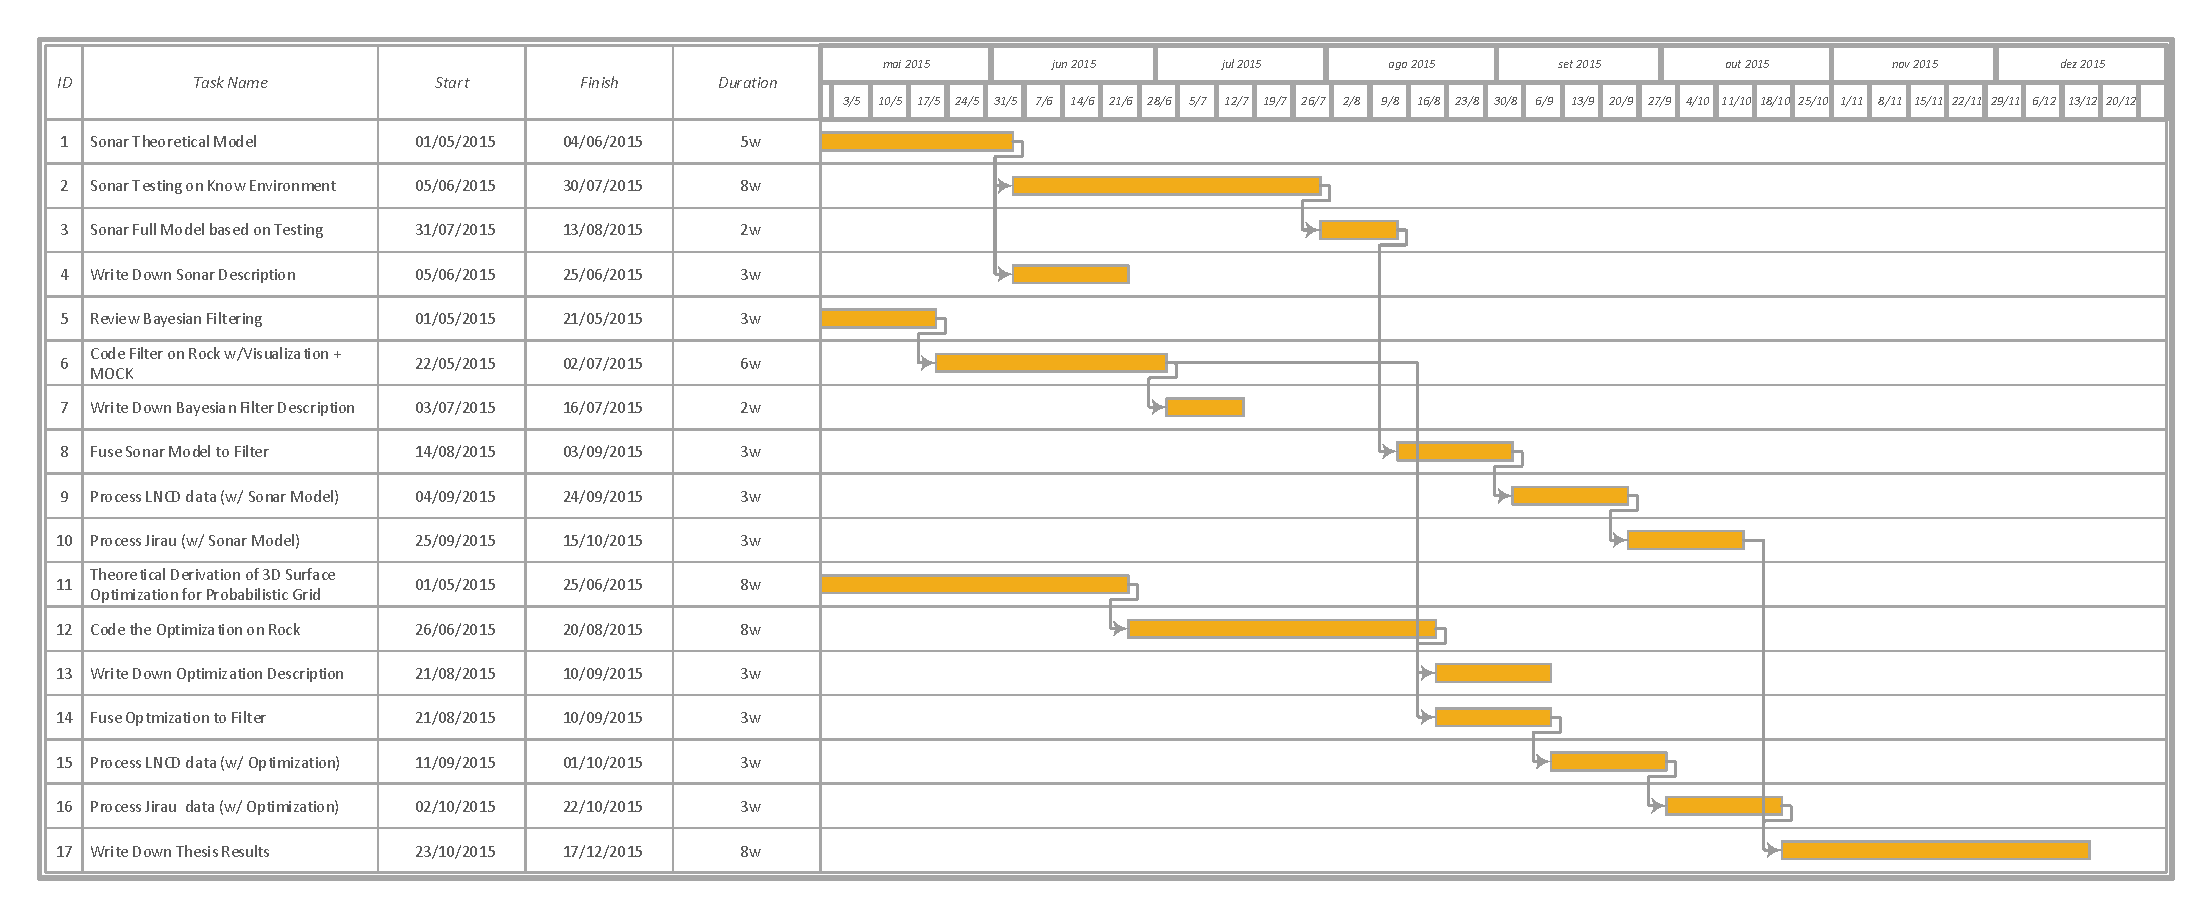
\includepdf[landscape=true,pagecommand=\section{Timetable and
milestones}]{TimeTable.pdf}
\end{landscape}
\section{Conclusion}

This master thesis proposal has described a less than a year full-time plan for
study and implementation of a underwater mapping system. So to be able to
scrutinize state of the art technologies to apply on a poorly explored
condition, that is the full 3D environment. And even, based on these
technologies, tailor a new algorithm to enhance the outcome. Besides the
theoretical realizations, it is committed to provide results based on real-world
data from UHE Jirau (the Jirau power plant).

\bibliographystyle{coppe}
\nobibliography{SoundPhysics,MathBackground,DiscreteSpace,Mapping,Related,Octomap}

\end{document}